\documentclass[12pt,a4paper,titlepage]{article}
\usepackage[utf8]{inputenc}
\usepackage[finnish]{babel}
\usepackage{setspace}
\usepackage{subcaption}
\usepackage{fancyhdr}
\usepackage[top=1in, bottom=1in, left=1in, right=1in]{geometry}
\usepackage{float}
\usepackage{pdfpages}
\usepackage{enumitem}

\usepackage{hyperref}
\hypersetup{pdfborder={0 0 0}}
\onehalfspacing
\cfoot{}
\rhead{\thepage}
\lhead{\leftmark}

\title{Tsoha\\ Kurssikysely \vspace{0.5em}}
\author{Anni Järvenpää}
\date{\today}

\begin{document}
\maketitle

% Sisällysluettelo
\newpage
\tableofcontents
\thispagestyle{empty}
\newpage
\setcounter{page}{1}
\parskip=1em \advance\parskip by 0pt plus 2pt
\pagestyle{fancy}
\cfoot{\thepage}

%%%%%%%%%%%%%%% Oleellinen sisältö alkaa%%%%%%%%%%%%%%%
\section{Johdanto}
Työn tavoitteena on toteuttaa kurssikyselyjärjestelmä, jonka avulla opiskelijoilta voidaan kerätä palautetta kursseista. Järjestelmää voidaan käyttää koko tiedekunnassa ja kyselyt sisältävätkin sekä koko tiedekunnan laajuisia kysymyksiä että laitos- ja kurssikohtaisia kysymyksiä. Kysymysten vastaukset voivat olla avoimia tai ne voidaan valita numeroasteikolta tai muusta annetusta arvojoukosta.

Kurssin luennoitsija voi lisätä, poistaa ja muokata kurssikohtaisia kysymyksiä ja laitoksen ja tiedekunnan hallintohenkilöstö niiden kysymyksiä. Samoin uusille kursseille voidaan luoda uusia kyselyitä ja vanhoja voidaan poistaa. Kyselyn muokkaaminen tai poistaminen edellyttää kuitenkin, ettei kysely ole parhaillaan käynnissä.

Laitos ja tiedekunta voivat hakea yhteenvedon kurssin tai kurssien kysymysten tuloksista kuten vastaajamääristä tai tiettyyn kysymykseen saaduista vastauksista. Kurssin pitäjä saa järjestelmästä yksinkertaisen raportin kyselyn tuloksista aina halutessaan.


\section{Yleiskuva järjestelmästä}
\subsection{Käyttötapaukset ja käyttäjät}
Järjestelmää käyttävät opiskelijat, opettajat ja laitoksen sekä tiedekunnan hallintohenkilöt. Näistä kaikki voivat kirjautua järjestelmään ja tarkastella kyselyitä. Näkyvät kyselyt ja niille tehtävissä olevat operaatiot riippuvat kuitenkin käyttäjäryhmästä.

Ainoastaan opiskelijat voivat vastata kyselyihin ja he näkevät kyselyt vain sellaisista kursseista, joilla he ovat parhaillaan.

%\begin{description}[style=nextline]
%	\item[Tiedekunnan hallintohenkilo] 
%	\item[Laitoksen hallintohenkilo] fds
%	\item[Opettaja] fdas
%	\item[Opiskelija] fdas
%\end{description}

%Heistä kaikki voivat kirjautua järjestelmään ja selata kyselyjä. Lisäksi jokaisella käyttäjäryhmällä on 

%Näistä kaikki voivat kirjautua järjestelmään ja tarkastella kyselyitä, joskin näkyvien kyselyiden määrä riippuu käyttäjästä. Lisäksi hallintohenkilöt ja opettajat pystyvät tarkastelemaan kyselyjen tuloksia käyttäjäryhmän määräämällä tarkkuudella sekä muokkaamaan omalle organisaatiotasolleen spesifejä kysymyksiä. Laitoksen hallintohenkilöstö luo ja ylläpitää kursseja, minkä jälken kurssin vastuuopettaja pystyy luomaan, muokkaamaan ja poistamaan omiin kursseihinsa liittyviä kyselyitä.

\begin{figure}
   \centering
   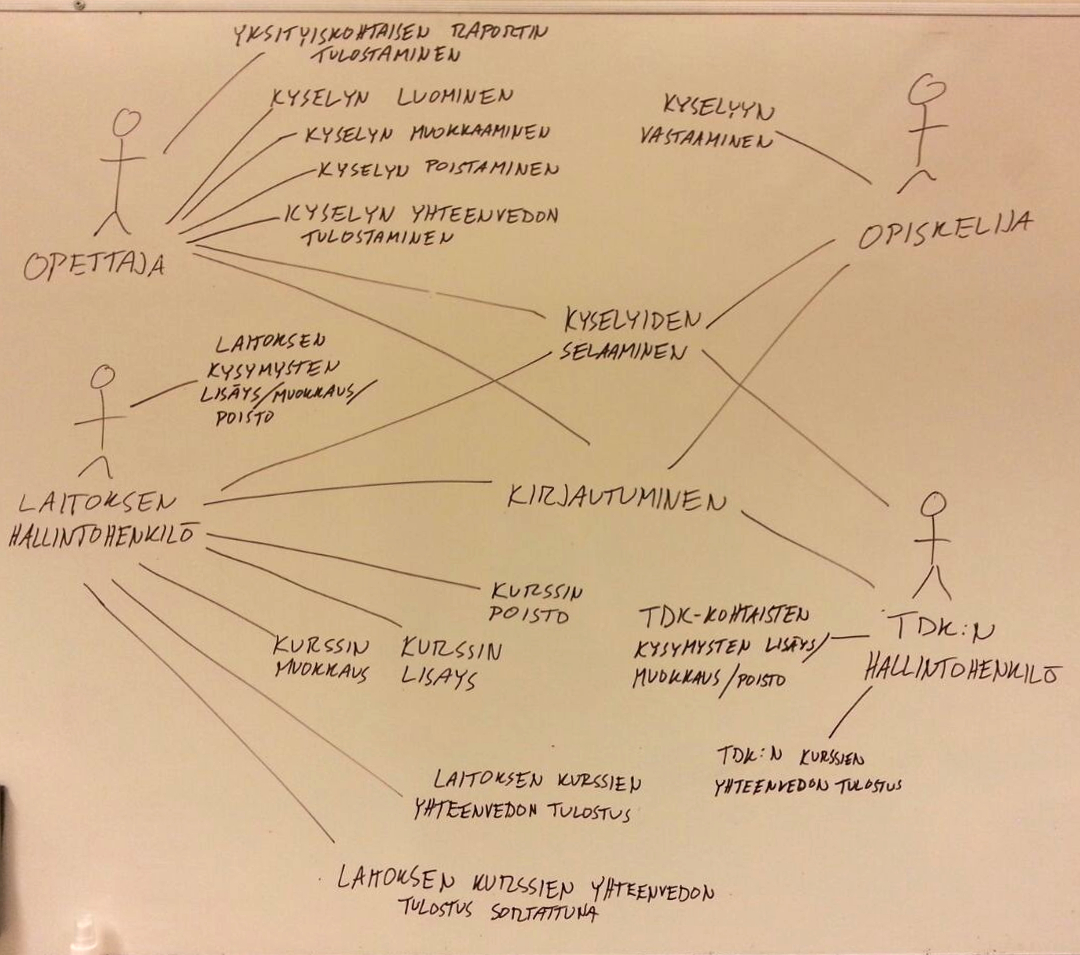
\includegraphics[width=\textwidth]{kuvat/kayttotapauskaavio.jpg}
   \caption{No kuvahan se siinä}\label{fig:kayttotapauskaavio}
\end{figure}




\section{Järjestelmän tietosisältö}

\section{Relaatiotietokantakaavio}

\section{Järjestelmän yleisrakenne}

\section{Käyttöliittymä ja järjestelmän komponentit}

\section{Asennustiedot}

\section{Käynnistys- ja käyttöohje}



%%%%% Sisältö loppuu, lähdeluettelo %%%%%
\bibliographystyle{plain}
\small
\bibliography{lahteet}

\appendix
%\newpage
\section{Tärkeä liite}
Lorem ipsum.
\newpage



\end{document}
